\section{Game library}

\begin{frame}{2D games}
	\begin{itemize}
		\item 2D game library implemented by Malte Sehmer (bachelor thesis)
		\item Supports sprites (loaded from bitmap files) and animations
		\item Collision detection based on rectangle colliders (ploygon colliders are conceptually implemented)
		\item Linear and accelerated movements are implemented (e.g. gravity)
	\end{itemize}
	\begin{minipage}{0.49\textwidth}
		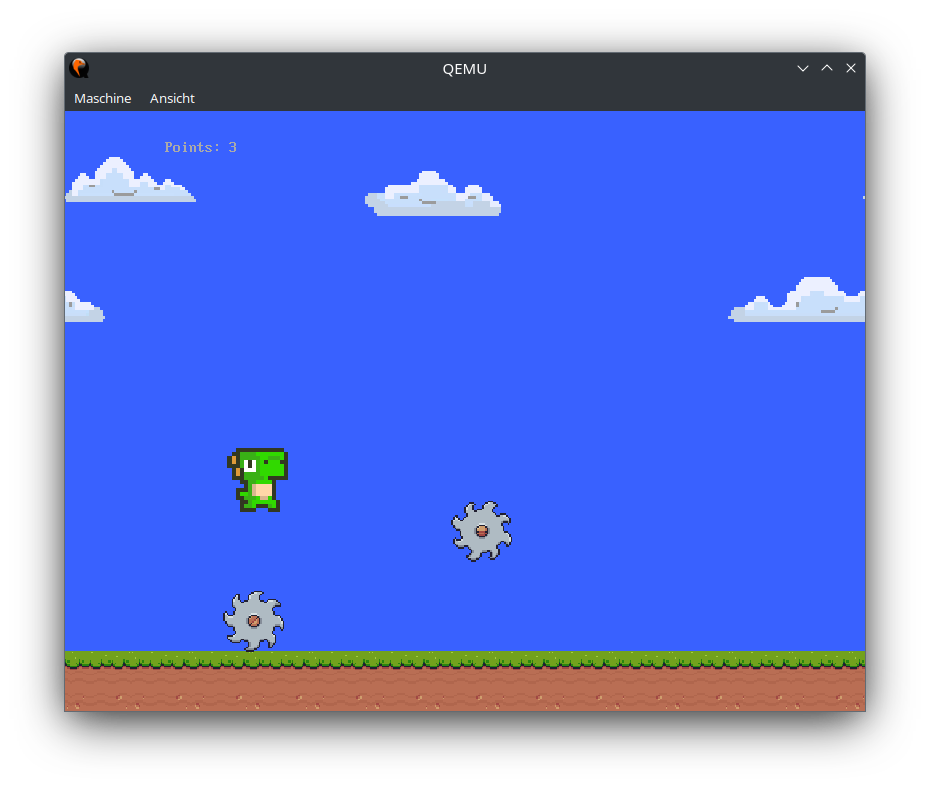
\includegraphics[width=0.95\textwidth]{img/dino}
	\end{minipage}
	\begin{minipage}{0.49\textwidth}
	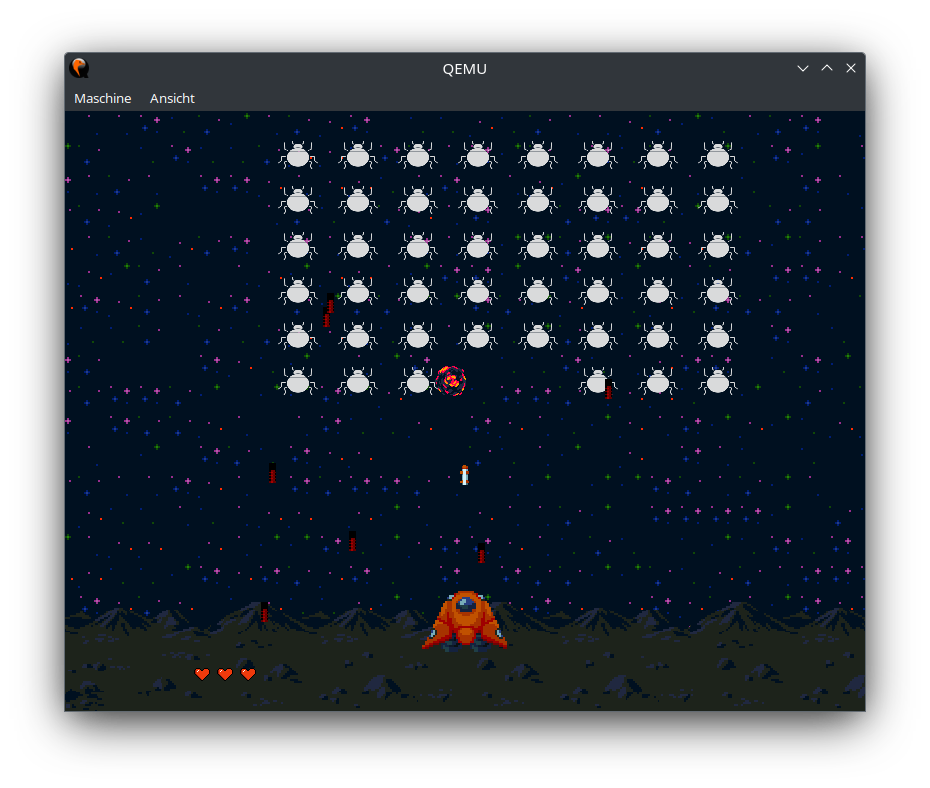
\includegraphics[width=0.95\textwidth]{img/bug}
	\end{minipage}
	\pause
	\begin{center}
		\textbf{But can it run Crysis?}
	\end{center}
\end{frame}

\begin{frame}{3D games - Work in Progress}
	\begin{itemize}
		\setlength\itemsep{1em}
		\item 3D game library implemented by Richard Schweitzer (bachelor thesis)
		\item Supports wireframe 3D-objects loaded from text files
		\item Collision detection based on spheres
	\end{itemize}
	\begin{minipage}{0.49\textwidth}
		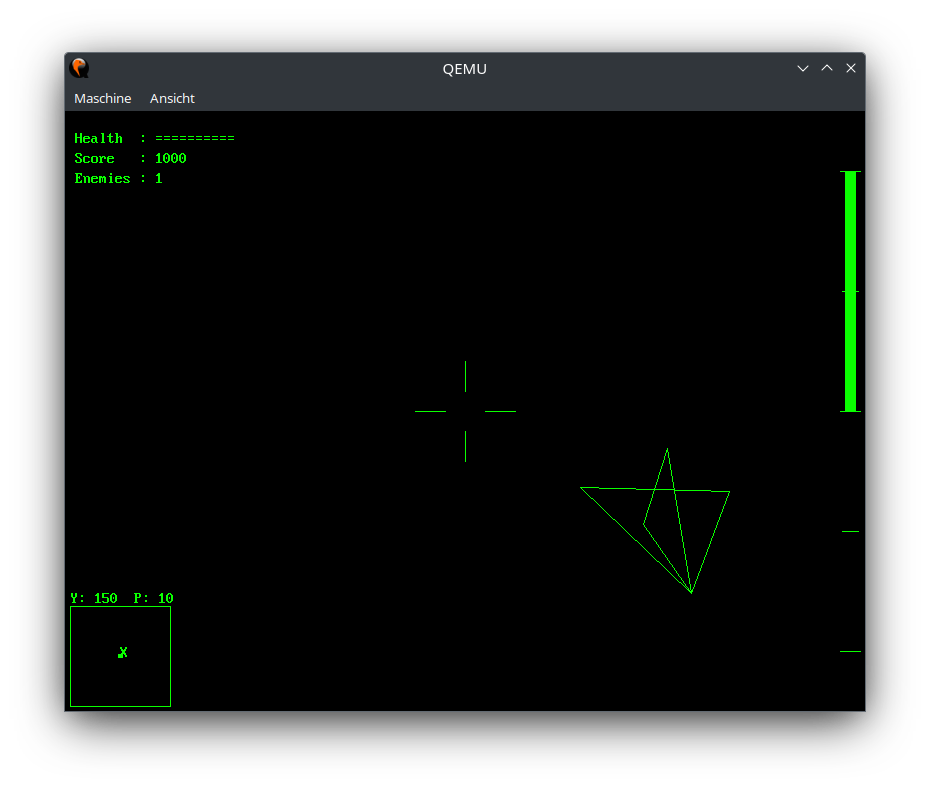
\includegraphics[width=0.95\textwidth]{img/battlezone1}
	\end{minipage}
	\begin{minipage}{0.49\textwidth}
		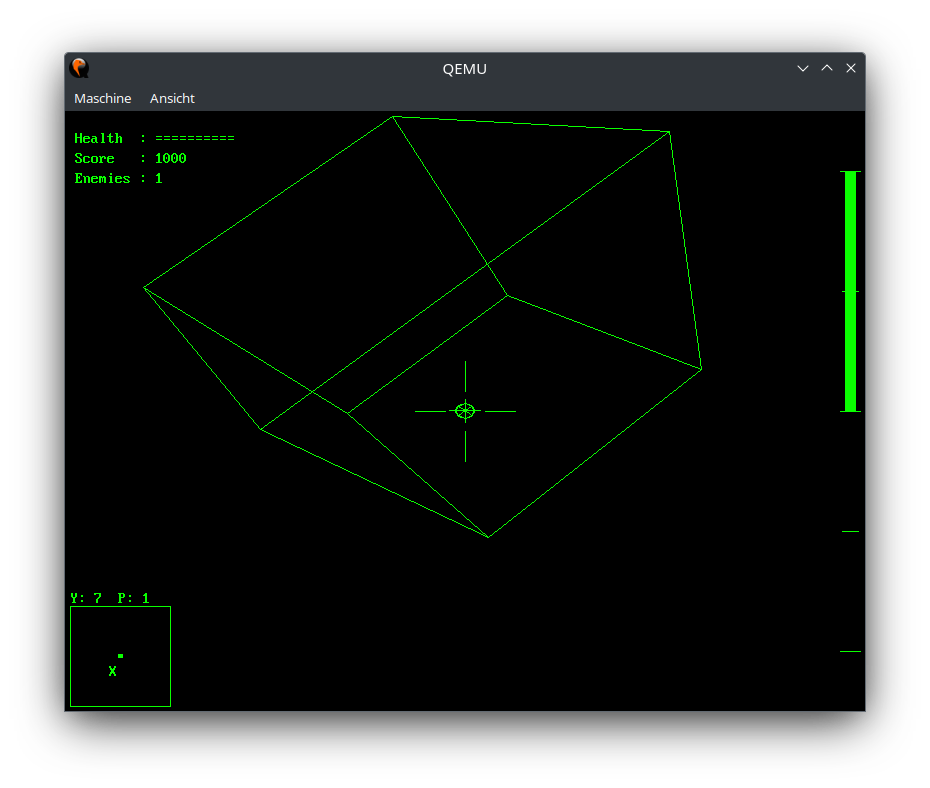
\includegraphics[width=0.95\textwidth]{img/battlezone2}
	\end{minipage}
\end{frame}
